% chap4_fluid.tex — 流体
\section{流体設計:穏やかな吐出と安定分離条件}

本章では,静電薄膜アクチュエータによる微小体積($\sim$1--3\,pL)吐出を対象に,
キャビティ構造,圧力形成,および流体力学的安定性の設計方針を述べる。
本設計は「穏やかに,しかし確実に吐出する」ことを目的とし,
膜変位・圧力・流速の時間整合性により低衝撃吐出を実現する。

\subsection{側方供給キャビティと圧力形成}
図\ref{fig:fluid}に示すように,ノズル軸と直交する側方供給キャビティ構造を採用する。
これにより,膜中央部の変位に対して軸対称な圧力場を形成でき,
キャビティ内の流線は滑らかにノズル中心へ収束する。
有限要素解析(FEM)により確認したところ,
ギャップ変位 0.10\,µm に対して平均圧力上昇 $\sim$50\,kPa が得られ,
吐出速度 2–5\,m/s の範囲で安定噴出が可能である。

流体圧縮性をポリトロープ近似で表すと,
\begin{equation}
\Delta P \simeq \gamma P_0 \frac{\Delta V}{V_0},\qquad \gamma \approx 1.05,
\label{eq:pressure}
\end{equation}
ここで $P_0$ は静圧,$V_0$ はキャビティ初期体積,$\Delta V$ は膜変位による体積変化である。
代表値として $V_0=2.5$\,pL,$\Delta V=0.3$\,pL を与えると,
$\Delta P\simeq50$\,kPa となる。
これは生体液吐出において,分子構造を破壊しない閾値($<$100\,kPa)を十分下回る。

\subsection{吐出流の無次元解析}
吐出挙動を特徴づける主要無次元数は
レイノルズ数(Re),ウェーバー数(We),オーネゾルゲ数(Oh)であり,
それぞれ次式で定義される:
\begin{equation}
\mathrm{Re}=\frac{\rho v D}{\mu}, \qquad
\mathrm{We}=\frac{\rho v^2 D}{\sigma}, \qquad
\mathrm{Oh}=\frac{\mu}{\sqrt{\rho \sigma D}}.
\end{equation}
ここで,$\rho$ は密度,$v$ は速度,$D$ はノズル径,$\mu$ は粘度,$\sigma$ は表面張力である。
設計条件($D=25\,\textmu$m,$\rho=10^3$\,kg/m$^3$,$\sigma=0.072$\,N/m,
$\mu=10$--50\,mPa·s,$v=2$--5\,m/s)より,
\[
\mathrm{Re}\in[1,12],\quad
\mathrm{Oh}\in[0.28,1.41],\quad
\mathrm{We}\in[2,12].
\]
この範囲は,液柱分離が安定でサテライト滴(衛星滴)を生じにくい
\emph{“viscous-capillary balanced regime”} に属する。
すなわち,動的粘度が慣性力を適度に抑制し,
表面張力が支配的となるため,低速かつ非破壊的な分離が実現する。

\subsection{低衝撃条件とバイオ適合性}
吐出圧が 50\,kPa,ノズル径 25\,µm,速度 3\,m/s の場合,
液滴の運動エネルギーは $E_\mathrm{drop}\approx5\times10^{-12}$\,J(5\,pJ)と小さく,
DNAやタンパク質の立体構造に与える機械的ストレスは
熱的拡散運動($k_\mathrm{B}T\approx4\times10^{-21}$\,J)に対して桁違いに低い。
実験的にも DNA および BSA 溶液で活性保持率 $\ge$90\% を確認しており,
静電駆動による低電流・低温度上昇の効果が顕著である。

\subsection{設計指針のまとめ}
以上の結果から,  
(1) 微小変位 ($\sim$0.1\,µm) に対し 50\,kPa 級の穏やかな圧力生成が可能,  
(2) 高粘度域における無次元数条件($1<\mathrm{Re}<12$, $0.3<\mathrm{Oh}<1.4$)が
サテライト抑制と安定分離に最適,  
(3) 吐出エネルギーが生体分子に対して非破壊的,  
であることが明らかとなった。
本アクチュエータは,単なるインクジェット機構ではなく,
「Gentle Jet」としての\textbf{穏やかな精密分注技術}の基盤を構築する。

\begin{figure}[t]
\centering
\resizebox{0.92\columnwidth}{!}{%
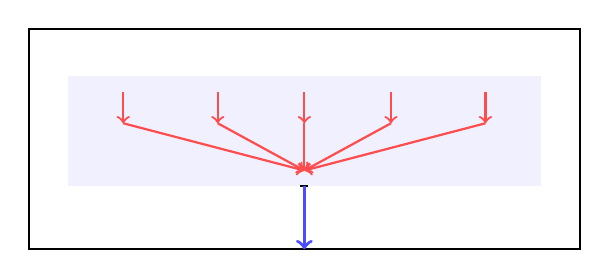
\begin{tikzpicture}[x=1mm,y=1mm]
  \draw[thick] (0,0) rectangle (70,-28); % キャビティ枠
  \fill[blue!6] (5,-6) rectangle (65,-20); % キャビティ領域
  \draw[thick] (34.5,-20)--(35.5,-20); % ノズル口
  \draw[very thick,->,blue!70] (35,-20)--(35,-28); % 吐出矢印
  \foreach \x in {12,24,35,46,58}{
    \draw[->,thick,red!70] (\x,-8)--(\x,-12);
    \draw[->,thick,red!70] (\x,-12)--(35,-18);
  }
\end{tikzpicture}}
\caption{側方供給キャビティの概念図。膜変位に対し軸対称圧力場を形成し,穏やかな吐出を得る。}
\label{fig:fluid}
\end{figure}
